\begin{titlepage}
\thispagestyle{empty}
\vspace*{3em}

% Logos top left and right
\noindent

\includegraphics[height=1.2cm]{figures/logo/eth_logo.png}
\hfill
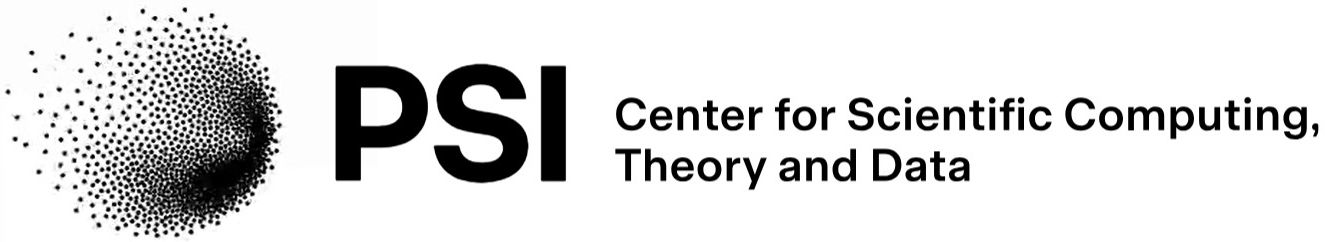
\includegraphics[height=1.57cm]{figures/logo/psi_logo.png}

{\sffamily 

\vspace*{4cm}
\begin{center}
\huge{\textbf{Theoretical MHD Modelling\\ of the Polomac Concept}}\\[0.9cm]
\Large{{Ideal MHD and Equilibrium Derivation and\\
       a Framework for Numerical Implementation}}
\end{center}

\vfill
\begin{center}
\begin{tabular}{ll}
\Large{{Author:}} & \Large{Nicola Rupf}\\[0.3em]
\Large{{Supervisor:\;\;}} & \Large{Dr. Andreas Adelmann}
\end{tabular}

\vspace{1.8cm}
\normalsize{\hspace{-1pt}Research Project, Department of Physics, 2026}
\end{center}

}%end ssf font family

\end{titlepage}

